\subsection{Example Chart: Sickness}
\begin{frame}[t]{Example Chart: Sickness }
\scriptsize
\begin{columns}[T, onlytextwidth]
\column{0.5\textwidth}
Mercury (L1) is Void of Course and does not aspect the 1st (so he's evil and impeded). \\
\vspace{0.2cm}
The \Moon\ is also Void of Course but she is \Trine\ the 1st House and she is the first to enter a new sign so we look to her first with \Mercury\ being made the sharer. \\
\vspace{0.2cm}

\textbf{\Moon\ in \Taurus\ \Trine\ 1st House} $\Rightarrow$ enters \Gemini \\
$\Rightarrow$ \Square\ \Venus\ in \Pisces\ and commits her disposition (no mention of reception) \\
\Venus\ $\Rightarrow$ \Sextile\ \Jupiter\ in \Taurus, MR by domicile \\
As \Jupiter\ cannot join with any other planet, he ends the disposition and becomes the final authority over the matter and determines the outcome.
\vspace{0.2cm}

\textbf{\Mercury\ in \Aries\ Void of Course} $\Rightarrow$ \Taurus \\
$\Rightarrow$ \Sextile\ \Venus\ \Pisces\ who receives him from \Taurus \\
\Venus\ $\Rightarrow$ \Trine\ \Jupiter\ in \Taurus\, MR by domicile \\
And again, \Jupiter\ is the end of the disposition chain, supporting what the \Moon\ indicated.
\vspace{0.2cm}

\Jupiter, a benefic, as the final arbiter of the disposition promises "health and quiet" and the end of the illness after a prolonged period (due to the VOC's) but we are told that from the time of \Venus\ accepting the \Moon's disposition to her joining with \Jupiter, the person would have gradually strengthened, with the illness leaving him completely once \Venus\ separates from \Jupiter\ by one minute.

%\column{0.01\textwidth}
%\rule{.1mm}{.35\textheight}

\column{0.5\textwidth}
{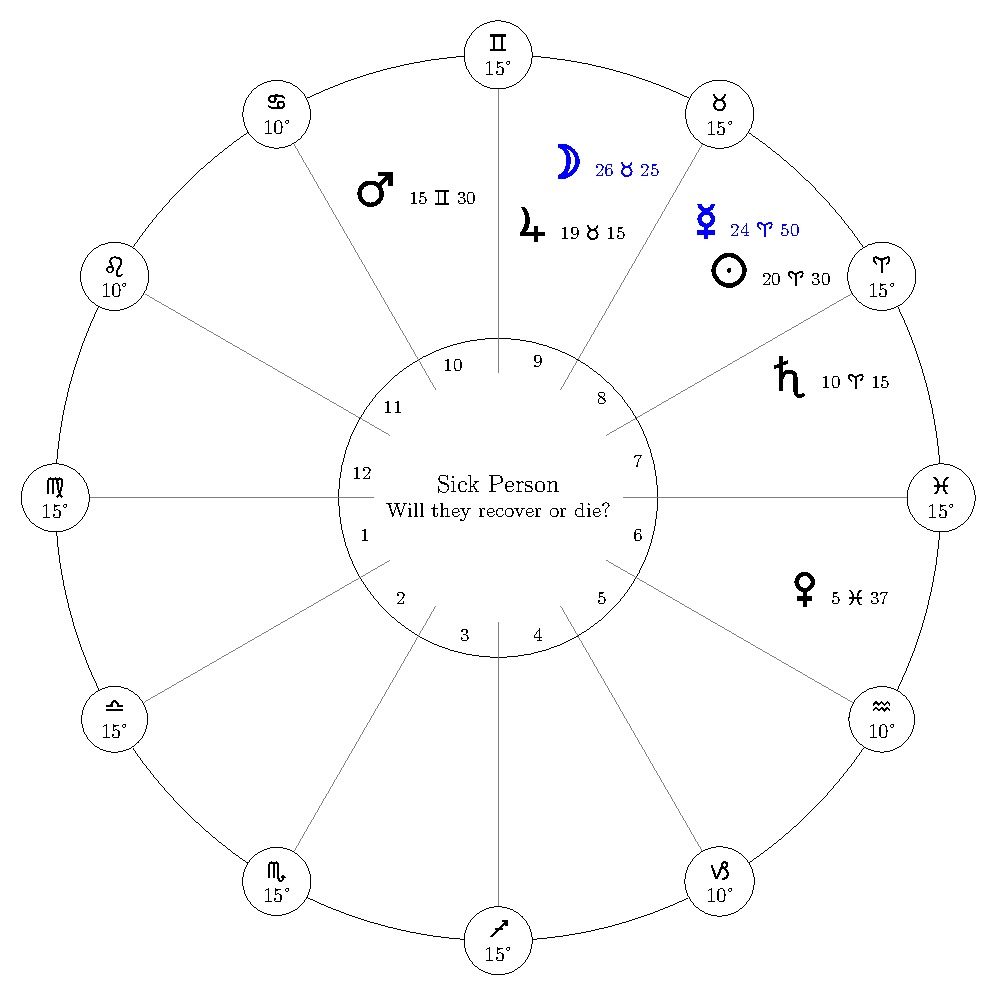
\includegraphics[width=0.9\textwidth]{charts/21-chart-sickness}}

\begin{itemize}
\item[] \textbf{Outcome:} \\
\item[] \hspace{2em} because of reception, is fortunate and perfected
\end{itemize}
\end{columns}
\end{frame}
% ------------------------------------------------------------
\begin{frame}[t]{Example Chart: Sickness Continued}

\end{frame}